\documentclass{ecnuthesis}
% 模版选项:
% printMode     是否开启打印模式, 若缺省则为关闭, 反之则为开启
% 用法示例
% \documentclass[printMode]{ecnuthesis}   (开启打印模式, 适合双面打印)
% \documentclass{ecnuthesis}              (关闭打印模式, 适合提交电子版)

\ecnuSetup {
% 参数设置
% 允许采用两种方式设置选项:
%   1. style/... = ...
%   2. style = { ... = ... }
% 注意事项:
%   1. 请勿在参数设置中出现空行
%   2. "=" 两侧的空格将被忽略
%   3. "/" 两侧的空格不会被忽略
%   4. 请使用英文逗号 "," 分隔选项
%
% info 类用于输入论文信息
    info = {
        title = {面向移动终端的可穿戴动态心电图的智能监测应用},
        % 中文标题
        %
        titleEN = {Intelligent Monitoring Application of Wearable Dynamic Electrocardiogram for Mobile Terminals},
        % 英文标题
        %
        author = {刘议临},
        % 作者姓名
        %
        studentID = {10195101428},
        % 作者学号
        %
        department = {软件工程学院},
        % 学院名称
        %
        major = {软件工程},
        % 专业名称
        %
        supervisor = {王丽苹},
        % 指导教师姓名
        %
        academicTitle = {副教授},
        % 指导教师职称
        %
        year  = 2023,
        % 论文完成年份
        %
        month = 4,
        % 论文完成月份
        %
        keywords = {\todo{todo}},
        % 中文关键词
        % 请使用英文逗号 "," 以分隔
        %
        keywordsEN = {\todo{todo}},
        % 英文关键词
        % 请使用英文逗号 "," 以分隔
        %
    },
% style 类用于简单设置论文格式
    style = {
        footnote  = plain,
        % 脚注编号样式
        % 可用选项:
        %   footnote = plain|circled
        % 说明:
        %   plain     脚注的编号仅为数字
        %   circled   脚注的编号为带圆圈数字 (仅限1-10)
        %   (默认选项为 plain )
        %
        numbering = arabic,
        % 章节编号样式
        % 可用选项:
        %   numbering = arabic|alpha|chinese
        % 说明:
        %   arabic    使用数字进行编号 (即理科要求)
        %   alpha     使用字母进行编号 (即外文要求)
        %   chinese   使用汉字进行编号 (即文科要求)
        %   (默认选项为 arabic )
        %
        fontCJK = fandol,
        % 中文字体选择
        % 可用选项:
        %   fontCJK = fandol|windows|mac
        % 说明:
        %   fandol    使用 TeX 自带的 fandol 字体
        %   windows   使用 Windows 系统内的字体 (中易)
        %   mac       使用 MacOS 系统内的字体
        %   (默认选项为 fandol )
        %
        fontMath = lm,
        % 数学字体选择
        % 可用选项:
        %   fontMath = lm|times
        % 说明:
        %   lm        使用 TeX 自带的 Latin Modern 数学字体
        %   times     使用 Times 风格的数学字体
        %   (默认选项为 lm )
        %
        bibResource = {./thesis-ref.bib},
        % 参考文献数据源
        % 由于使用的是 biber + biblatex , 所以必须明确给出 .bib 后缀名
        %
        logoResource = {./inner-cover(contains-font).eps},
        % 封面插图数据源
        % 模版已自带, 位于 ./inner-cover(contains-font).eps
        % 默认值为空
    }
}

% 需要的宏包可以自行调用
\usepackage[chapter]{easy-todo}
\usepackage{graphicx}
\usepackage{newfloat}
\usepackage{hyperref}

% https://tex.stackexchange.com/a/584994/254533
\captionsetup[figure][bi-second]{name=Figure}
\captionsetup[bi-second]{listtype+=Eng}
\DeclareFloatingEnvironment[fileext=lof2]{figureEng}[Figure][List of Figures]

\begin{document}

    \newcommand*{\app}{移动心电监测应用}


% 设置前置部分编号
    \frontmatter

% 中文摘要环境
    \begin{abstract}
        \todo{300到500字,要求概括地表述论文(设计)的研究背景、目的、研究方法、研究重点、结果和主要结论。}
    \end{abstract}

% 英文摘要环境
    \begin{abstractEN}
        \todo{中文摘要写完之后翻译一下}
    \end{abstractEN}

% 设置正文编号
    \mainmatter


    % TeXiFy 似乎无法正确解析 *.tex 和 thesis-ref.bib 的关联,导致误报 UnresolvedReference
%! suppress = UnresolvedReference


\chapter{绪论}\label{ch:intro}


\section{\app 的背景与意义}\label{sec:background}

\subsection{国内外心血管疾病现状}\label{subsec:disease}

根据中国国家心血管病中心出版的《中国心血管健康与疾病报告2021》\cite{Zhongguoxinxieguanjiankangyujibingbaogao20212022},目前中国人口心血管疾病的发病率和患病率均处于持续上升阶段,心血管疾病已成为居民死亡的首位原因;如图~\ref{fig:2019-death} 所示,2019年,中国农村、城市心血管疾病分别占疾病死因的46.74\%和44.26\%。心血管疾病给社会和居民带来的经济负担日益加重,且杀伤力越来越强。

\begin{figure}[!ht]
    \centering
    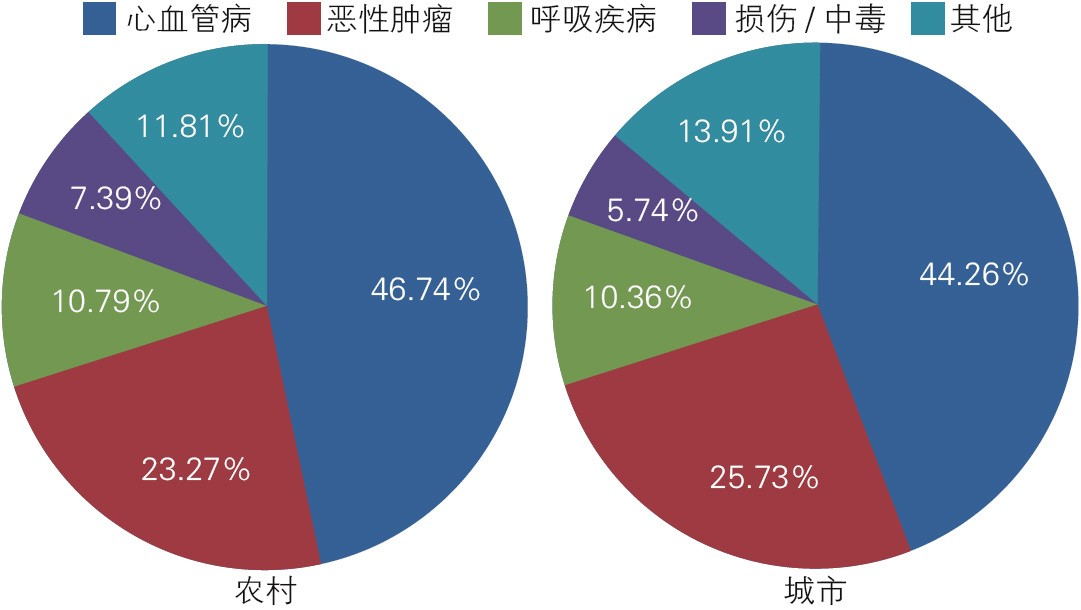
\includegraphics[width=.7\textwidth]{../assets/2019-death}
    \bicaption{2019年中国城乡居民主要疾病死因构成比\cite{Zhongguoxinxieguanjiankangyujibingbaogao20212022}}{Proportion of major causes of death among rural and urban in China in 2019}
    \label{fig:2019-death}
\end{figure}

不仅如此,根据世界卫生组织的统计\cite{CardiovascularDiseasesCVDs},心血管疾病也是全球的头号死因,每年死于心血管疾病的人数多于任何其它死因;2019年,估计有1790万人死于心血管疾病,占全球死亡总数的32\%。

同时,近年来新型冠状病毒(COVID-19)的爆发也加剧了心血管疾病的危害。证据显示,既往合并心血管疾病的患者更容易在新型冠状病毒感染后发展为重症患者,死亡风险更高,体征和症状更容易恶化\cite{zhangXinxingguanzhuangbingdufeiyanyuxinxieguanjibing2020}。

\subsection{心电监测的用途与原理}\label{subsec:monitoring}

尽早发现心血管疾病非常重要,这样就可以及时采取措施,减少疾病对患者健康的威胁\cite{CardiovascularDiseasesCVDs}。在各种心血管疾病的诊断方法中,心电图(Electrocardiogram,缩写为ECG)是最常用、最基本、最重要的一种,具有非侵入性、诊断快速、成本低廉、广泛可用等诸多优点\cite{Xinxieguanjibingzhenduanliuchengyuzhiliaocelue2007}。

心电图是对心电信号的记录。通过放置在皮肤上的电极可以检测到心脏的电活动,将电压与时间的关系绘制为二维图像就得到了心电图。

\subsection{常规心电图与动态心电图}\label{subsec:standard-holter}

心电图有两种主要类型:常规心电图(Standard ECG)和动态心电图(Holter ECG、Dynamic ECG或Ambulatory ECG)。

常规心电图,也被称为静息心电图(Resting ECG),是在患者保持静止状态时记录的心电图。常规心电图的记录需要在专业的医疗机构中进行,患者通常处于平躺状态,在四肢和胸部表面安装电极,电极检测心脏产生的电信号并将其传输到心电图仪器。常规心电图通常包含12个导联\footnote{这里的一个导联是指一对电极之间的电势差,比如II导联是指右臂电极和腿电极之间的电势差。另外,连接电极与心电图仪器的电缆也常被称为导联。本文中无特别说明的情况下,导联均指电势差而非电缆。},一次记录10秒,并打印在心电图纸上。如图~\ref{fig:ecg-paper-example} 所示是一张10秒12导联的常规心电图。

\begin{figure}[!ht]
    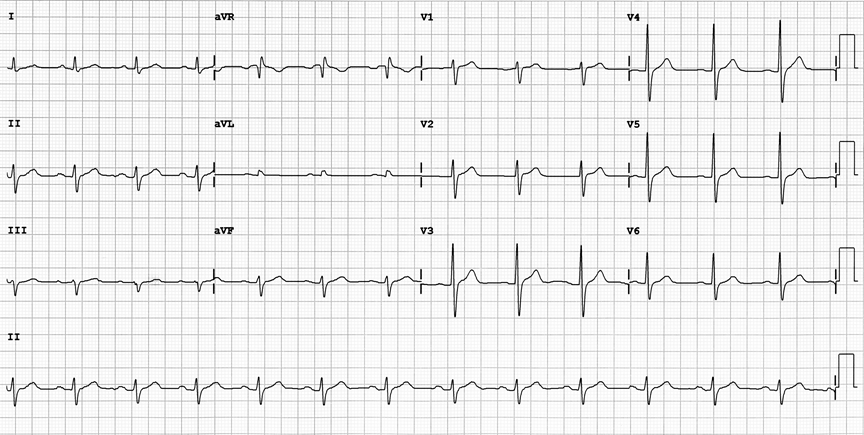
\includegraphics[width=\textwidth]{../assets/ecg-paper-example}
    \bicaption{一张10秒12导联的常规心电图}{A 10-second 12-lead standard ECG}
    \label{fig:ecg-paper-example}
\end{figure}

动态心电图则是在患者进行日常生活活动时记录的心电图。动态心电图的记录可以在几乎任何环境进行,只需要患者佩戴动态心电记录仪(Holter monitor)即可。动态心电记录仪是一种便携式可穿戴设备,可在较长时间内(24小时以上)记录心脏的电活动,有助于检出非持续性心律失常。统计显示,动态心电图在临床诊断中对心肌缺血及各种心律失常事件的检出率都明显高于常规心电图\cite{zhengDongtaixindiantuyuchangguixindiantuzhenduanguanxinbinghuanzhexinjiquexiejixinlushichangdelinchuangxiaoguobijiao2011}。

\subsection{\app 的意义}\label{subsec:app-significance}

动态心电图的数据量远远超过常规心电图,在显著提升了诊断精度的同时,也大幅提高了人工诊断的难度。人工进行大量数据的诊断识别,不仅使得医生过于疲劳、容易出错,也难以进行实时监测。于是,可以进行动态心电自动分析的\app 的需求就显而易见了。应用可以基于自动化的心电分析算法快速、准确地处理心电信号,为专业医疗人员节省时间,提高医疗服务的效率,降低医疗成本。使用\app 也更方便对患者进行实时监测,通过对心电数据进行实时分析可以及时发现患者的异常状况,为患者提供随时随地的医疗监护,降低心血管疾病对患者健康的威胁。


\section{相关技术与应用现状}\label{sec:status}

\subsection{动态心电自动分析技术现状}\label{subsec:automatic-analysis}

动态心电自动分析是指在采集到的动态心电信号的基础上,通过对其处理提取表征心脏状态的波形信息和特征参数,获取心脏工作状态的相关信息,然后利用这些特征信息分析、判别心电信号类型及所对应的疾病类型或健康水平,进而对心脏状态和健康状况进行预测\cite{jiXindianxinhaozidongfenxiguanjianjishuyanjiu2006}。

为了进行动态心电信号的自动分析,已经提出过许多相关算法。比如最著名的Pan-Tompkins算法\cite{panRealTimeQRSDetection1985}可以实时提取出心拍的位置,被广泛用于实时心率检测。U-Net模型\cite{ronnebergerUNetConvolutionalNetworks2015}作为一种生物医学图像分割模型也可以用于心拍提取,虽然无法实时给出结果,但在准确度等方面相较Pan-Tompkins等传统算法表现更好。基于ResNet\cite{heDeepResidualLearning2015}则可以训练心拍分类模型,用于自动识别每个心拍是否正常以及异常类型。

\subsection{国内外\app 现状}\label{subsec:app-status}

当前国内外已有不少\app ,其中一些使用了人工编写的传统心电分析算法\cite{zhengJiyukechuandaishebeideyidongjianhuAPP2019,wuYidongxindianjiancexitongdeyanjiuyushixian2018,chenYidongxindianxinxijianhuxitongjixindianjiancesuanfadeyanjiu2018,heJiyuyidongpingtaidexindianjianceyiliaoxitongdeshixian2017,gradlRealtimeECGMonitoring2012,wenRealtimeECGTelemonitoring2008},包括自适应双阈值法\cite{chenYidongxindianxinxijianhuxitongjixindianjiancesuanfadeyanjiu2018}、Pan-Tompkins算法\cite{gradlRealtimeECGMonitoring2012}以及一些原创的或基于已有算法改进的未命名的算法等;另一些\app 则使用了深度学习模型\cite{wangJiyushenduxuexideyidongyuanchengxindianjiancexitongshejiyushixian2020,singhSmartECGMonitoring2022,chenJiyushenduxuexidexindianfenximoxingdeshejiyuyouhua2021,liuJiyuyidongzhongduanfenxidekechuandairouxingxindianjiancexitong2021,wangEnablingSmartPersonalized2014,jinPredictingCardiovascularDisease2009}。

使用了深度学习模型的这些\app 按其整体架构可以大致分为两类:一类是在移动端只对数据进行简单统计处理,完整的算法模型则部署于服务端\cite{wangJiyushenduxuexideyidongyuanchengxindianjiancexitongshejiyushixian2020,singhSmartECGMonitoring2022},患者如果想获取完整的分析报告,则需要将数据上传至服务端后,等待服务端分析完成;这种应用架构的主要缺点是,患者能在移动端立即获取的结果较少,而完整分析结果可能因为网络质量差、服务端算力不足等原因而有较大延迟;另外,虽然患者不需要在自己的设备上运行相关算法,节省了一定开销,但上传与下载数据消耗的电量与流量成本不可忽视。另一类应用则采用了边缘计算架构,将深度学习模型部署在移动端,数据分析直接在移动端进行\cite{chenJiyushenduxuexidexindianfenximoxingdeshejiyuyouhua2021,liuJiyuyidongzhongduanfenxidekechuandairouxingxindianjiancexitong2021,wangEnablingSmartPersonalized2014,jinPredictingCardiovascularDisease2009},这样可以缩短延迟,节省带宽,并节省了高算力服务器的成本;然而,已有的少数此类应用都只实现了极简单的功能,旨在以演示应用验证模型正确性,并没有进行完整的应用开发,如图~\ref{fig:demos} 所示;此外,这些简单的演示应用均只进行了单一操作系统的开发。

\begin{figure}[!ht]
    \subcaptionbox{陈桂琛的应用\cite{chenJiyushenduxuexidexindianfenximoxingdeshejiyuyouhua2021}}{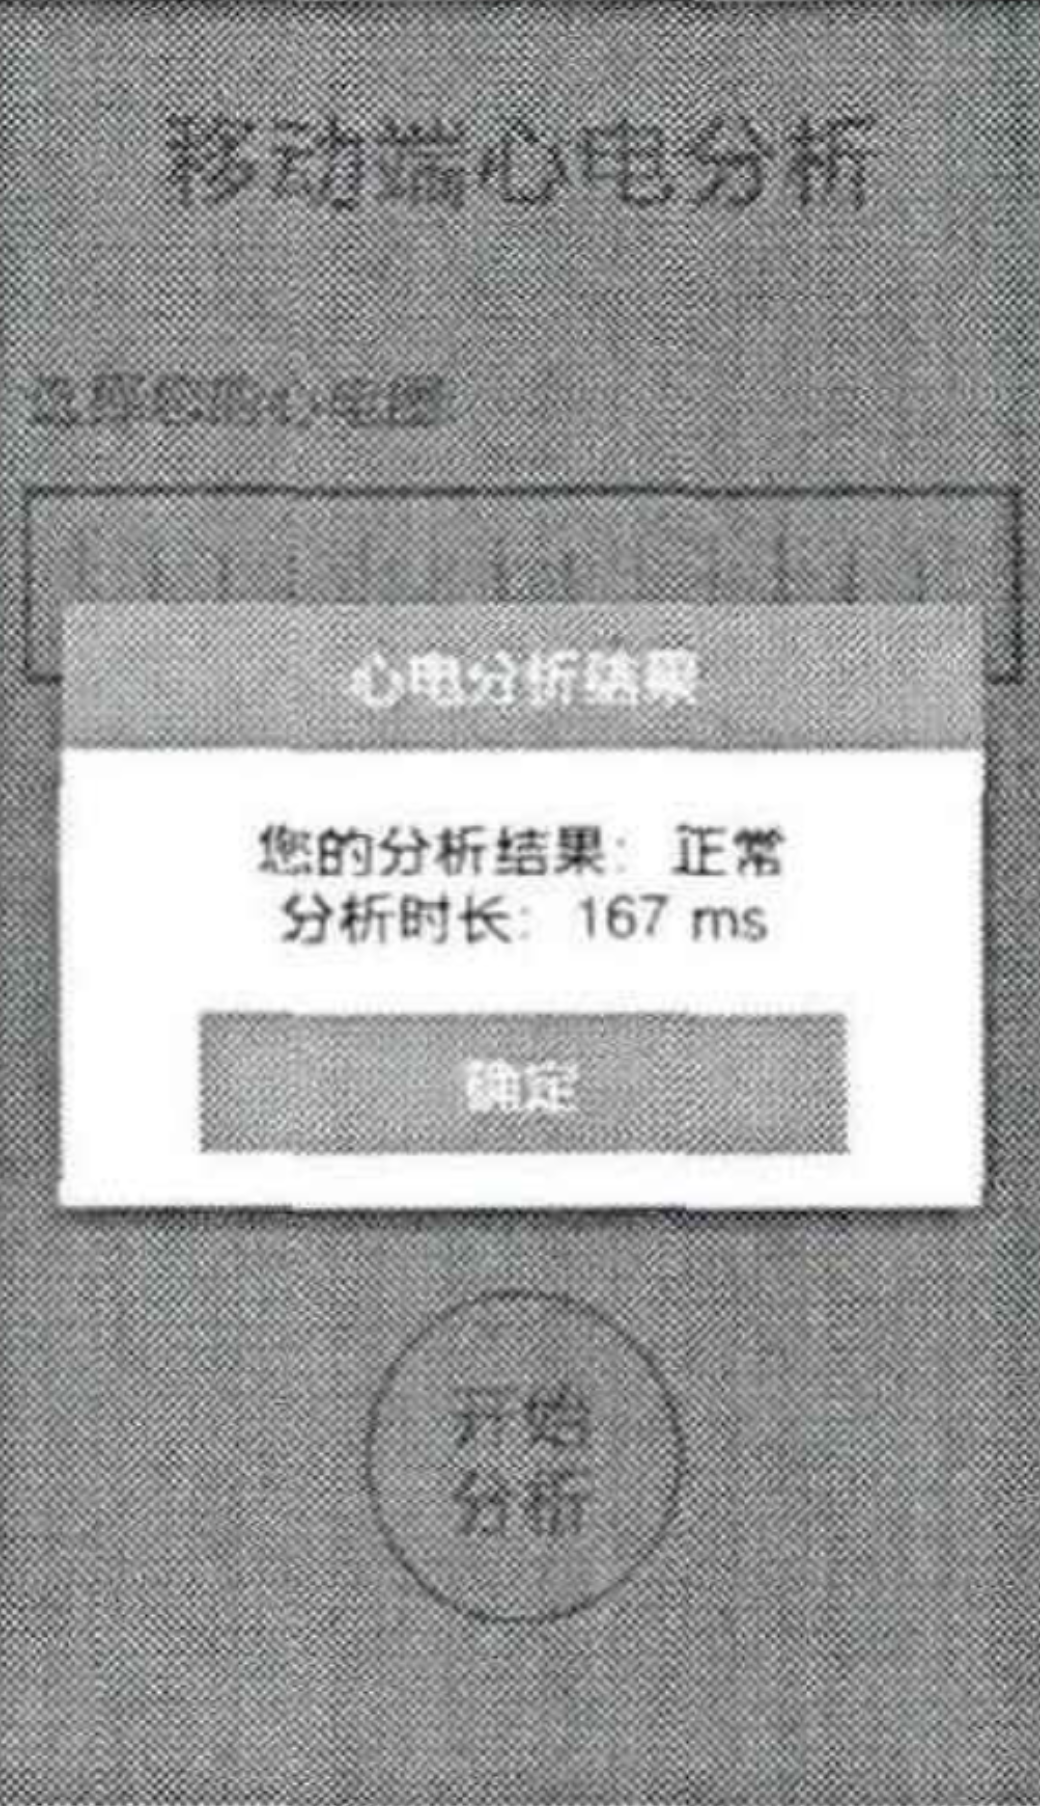
\includegraphics[height=9cm]{../assets/demo-0}}
    \subcaptionbox{刘荟的应用\cite{liuJiyuyidongzhongduanfenxidekechuandairouxingxindianjiancexitong2021}}{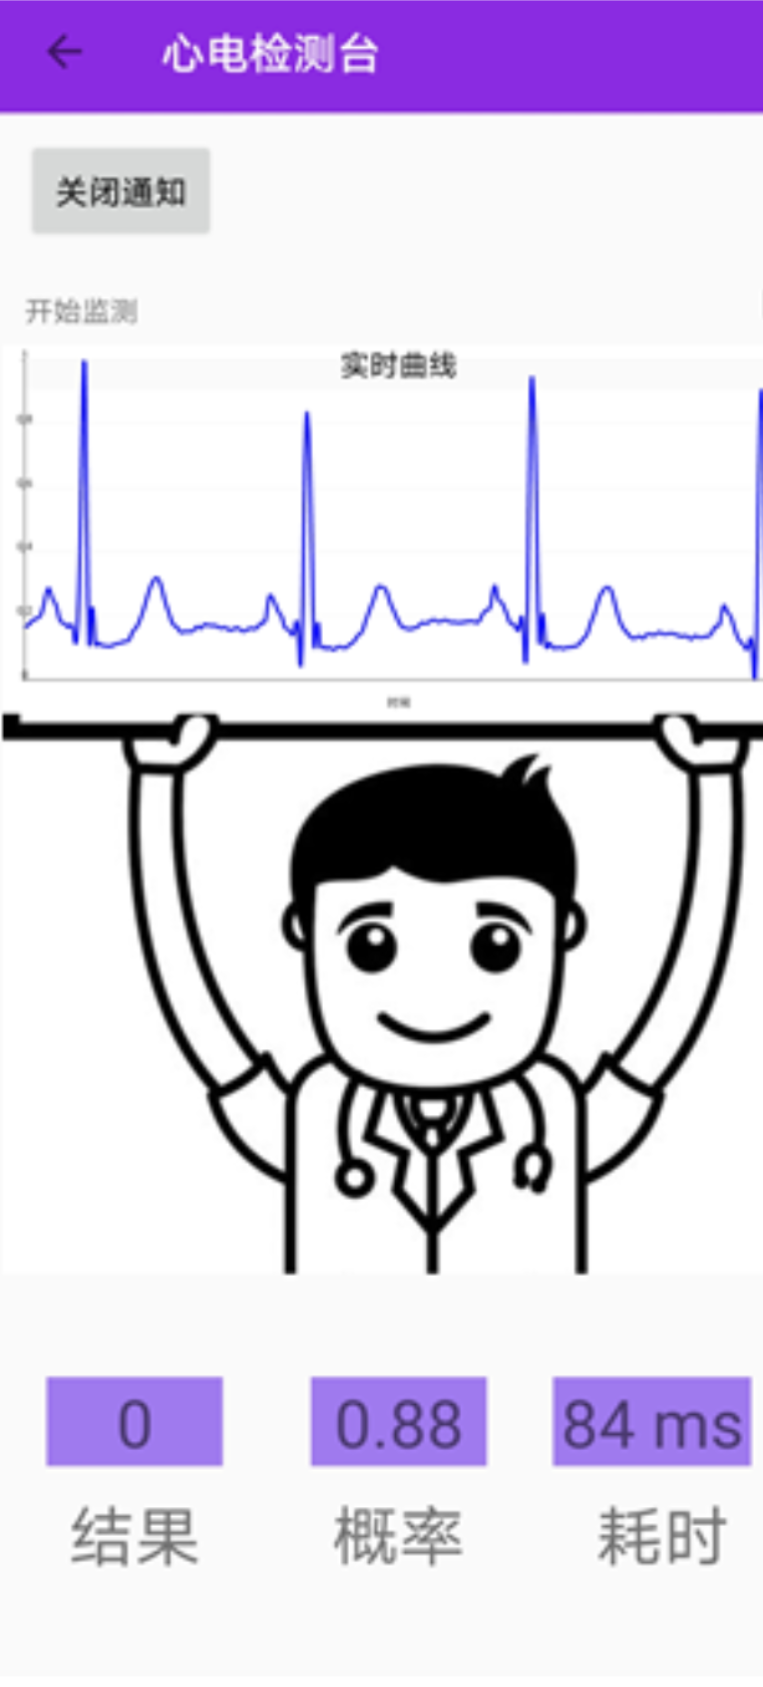
\includegraphics[height=9cm]{../assets/demo-1}}
    \subcaptionbox{Zhanpeng Jin等的HeartToGo\cite{jinPredictingCardiovascularDisease2009}}{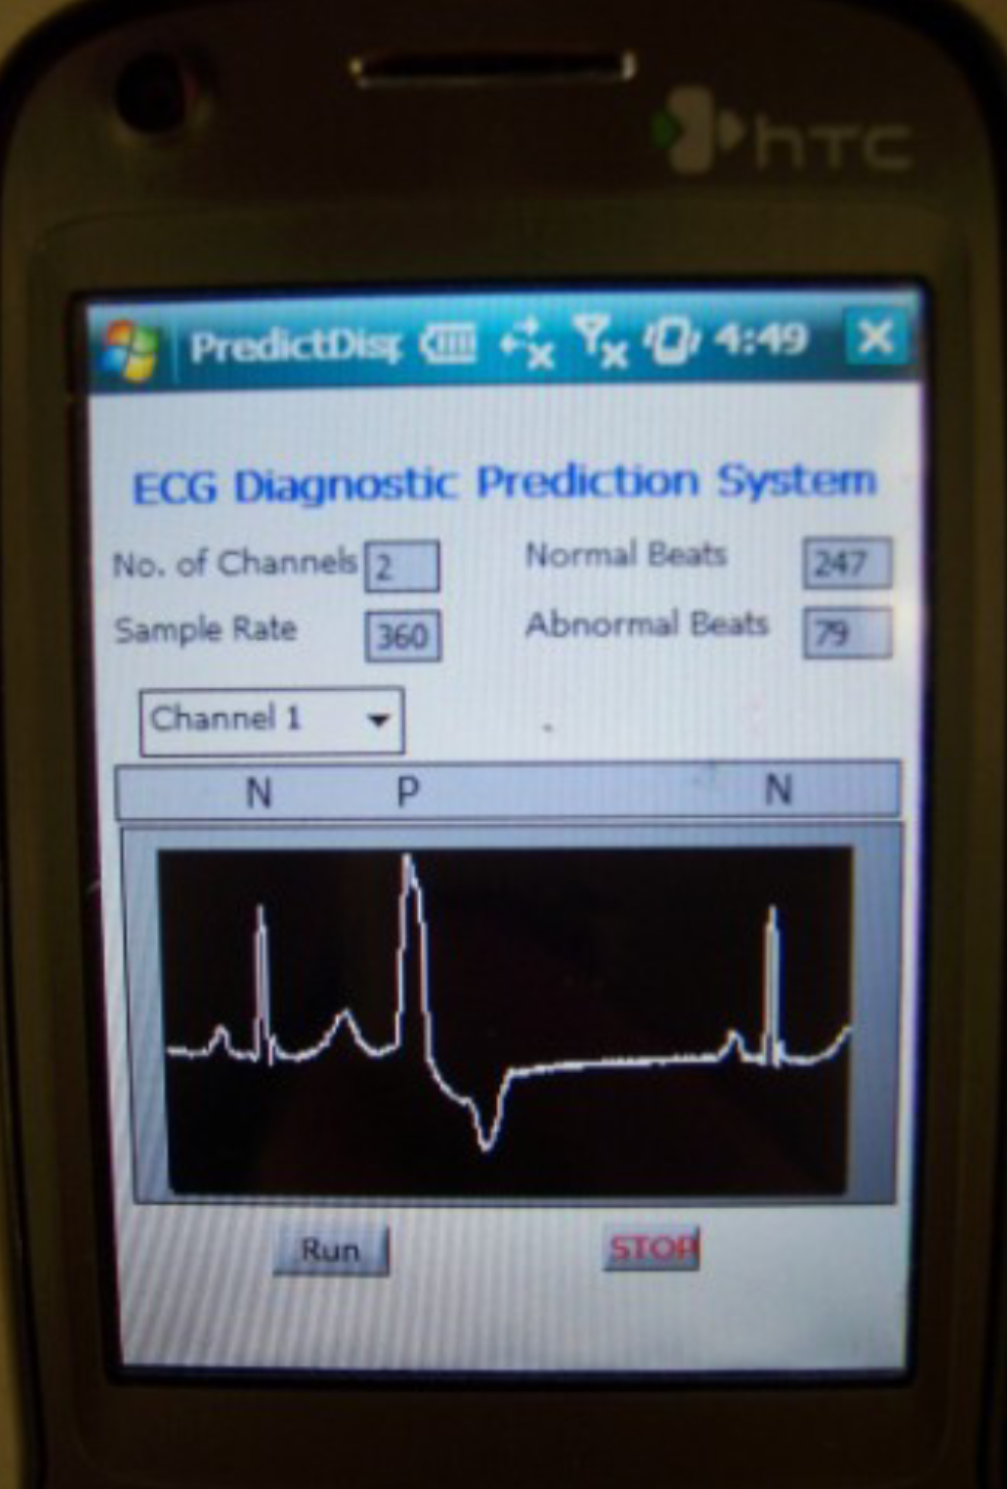
\includegraphics[height=9cm]{../assets/demo-2}}
    \bicaption{一些仅为验证模型而开发的简单演示应用}{Some demo apps only for model validation}
    \label{fig:demos}
\end{figure}


\section{本项目的主要工作}\label{sec:work}

本项目与~\ref{subsec:app-status} 节中所述的最后一类相似,也就是采用边缘计算架构,将深度学习模型部署在移动端,数据分析直接在移动端进行。本项目与上文提及的已有的同类应用的主要差别在于其选题来源于导师的心电图课题的子项目,是在已经基于PyTorch完成了相关算法模型\cite{songDongtaixindiantudezhinengjiancesuanfayanjiuyuyingyong2022}的情况下进行的,在项目之初就已有较好的人工智能算法模型的技术支撑。于是,相比于偏重算法研究而在实际的应用开发方面较为欠缺的其他项目,本项目的主要工作在于将已有的算法模型与移动应用开发技术进行整合,以实现一个较为完整的\app ,目标是最终投入到实际的生产环境中供患者使用。

在项目过程中,首先对应用的需求进行了分析,明确了应用的功能性需求和非功能性需求。然后为了满足需求进行了技术选型,明确了项目要使用的技术栈。之后对应用的整体架构和各个模块进行了设计。在开发阶段,完成了已有算法的移植与优化,以及应用程序本身的开发。最后,对应用进行了测试,以确保其可以满足需求。


\section{论文组织结构}\label{sec:structure}

本文分为7个章节,各章节的主要内容如下:

\begin{description}
    \item [1、绪论] 介绍了本项目的背景与意义、相关技术与应用现状、本项目的主要工作、本文的组织结构。
    \item [2、相关技术介绍] 对本项目使用的相关技术进行了介绍,包括Flutter相关的移动应用开发技术和算法相关的一些技术。
    \item [3、可穿戴动态心电监测应用的需求分析] 对应用进行了需求分析,明确了应用的目标用户、功能性需求、非功能性需求、项目可行性。
    \item [4、可穿戴动态心电监测应用的设计] 对应用的整体架构和各个模块以及数据库进行了设计。
    \item [5、可穿戴动态心电监测应用的开发] 介绍了应用的开发过程,包括开发环境与工具、算法的实现与移植、应用程序各个模块的实现等。
    \item [6、可穿戴动态心电监测应用的测试] 包含项目的测试环境、测试数据、测试方法、测试用例等。
    \item [7、总结与展望] 总结了本项目的主要工作,对未来的工作进行了展望。
\end{description}



    \chapter{相关技术分析与介绍}\label{ch:tech}

    \todo{技术方案(技术路线、技术措施),包括应用系统的架构和开发环境}


    \chapter{\app 的需求分析}\label{ch:requirement}

    \todo{todo}

    本应用的目标用户是佩戴可穿戴心电信号监测设备的院外患者,以中老年人为主。


    \chapter{\app 的设计}\label{ch:design}

    \todo{todo}


    \chapter{\app 的开发}\label{ch:development}

    \todo{todo}


    \chapter{\app 的测试}\label{ch:test}

    \todo{测试环境和测试数据的情况等。}


    \chapter{总结与展望}\label{ch:conclusion}

    \todo{todo}


% 正文后部分
    \backmatter
% 导入参考文献 (需要通过 latexmk 编译后才能显示)
    \PrintReference

% 附录环境
    \begin{appendix}

        \begingroup
        \renewcommand{\clearpage}{\relax}
        \listoftodos
        \endgroup

        \listoffigures
        \listoffigureEng


        \chapter*{部分插图的许可协议}\label{ch:license}

        文中使用的部分插图来自维基共享资源,相关信息列举于此。

        \section*{图\ref{fig:10sec-ekg-lead}}

        \begin{description}
            \item[作品名称:]10秒心电图纸
            \item[作者:]\href{https://zh.wikipedia.org/wiki/User:Kuyohong}{邱钰锋}
            \item[许可协议:]\href{https://creativecommons.org/licenses/by/4.0/}{署名-相同方式共享 4.0 国际 (CC BY-SA 4.0)}
            \item[作品链接:]\url{https://commons.wikimedia.org/wiki/File:10sec-ekg-lead.jpg}
            \item[是否对原始内容进行了更改:]否
        \end{description}

    \end{appendix}

% 致谢环境
    \begin{acknowledgement}
        \todo{此处撰写致谢词,主要感谢论文撰写过程中给予帮助的老师和同学,也可以感谢大学四年学习生涯中曾给予你重要帮助的人。请勿照抄。}
    \end{acknowledgement}

\end{document}
